%implementing document formatting:
\documentclass[12pt,twoside,a4paper]{report}

% Select encoding of your inputs
\usepackage[utf8]{inputenc}

% Make latex understand and use the typographic
% rules of the language used in the document.
\usepackage[english]{babel}

% Use the vector font Latin Modern which is going
% to be the default font in latex in the future.
\usepackage{lmodern}

% Choose the font encoding
\usepackage[T1]{fontenc}

% Use color in tables
\usepackage[table]{xcolor}
\usepackage{array}
\usepackage{multirow}

% Load a colour package
\usepackage{xcolor}
\definecolor{aaublue}{RGB}{33,26,82}  %<--define aaublue
\definecolor{white}{RGB}{255,255,255} %<--define white

% The standard graphics inclusion package
\usepackage{graphicx}

\makeatletter
  \g@addto@macro\@floatboxreset\centering %<--centering all figures
\makeatother

\usepackage{adjustbox}

% Set up how figure and table captions are displayed
\usepackage{float}
\usepackage{caption}
\usepackage{subcaption}
\captionsetup
{
  justification = justified,         %<--centering caption with multiple lines
  font          = footnotesize, %<--set font size to footnotesize
  labelfont     = bf            %<--bold label (e.g., Figure 3.2) font
}
\captionsetup[subfigure]
{
  justification = centering, %<--centering subfigure caption text
  singlelinecheck=false,
  font = footnotesize        %<--font size for subfigures
} 

% Enable row combination in tables
\usepackage{multirow}

% Make space between table lines and text
\renewcommand{\arraystretch}{1.5}

% Enable commands like \st (strike out) and \hl (high light)
\usepackage{soul}

% Make the standard latex tables look so much better
\usepackage{array,booktabs}

% Enable the use of frames around, e.g., theorems
% The framed package is used in the example environment
\usepackage{framed}
\usepackage{colortbl}
\usepackage{longtable}
\usepackage{xcolor}
\usepackage{textcomp}

%-------MATHEMATICS---------------------------------
% Defines new environments such as equation,
% align and split 
\usepackage{amsmath}
\usepackage{relsize}
% Adds new math symbols
\usepackage{amssymb}
% Use theorems in your document
% The ntheorem package is also used for the example environment
% When using thmmarks, amsmath must be an option as well. Otherwise \eqref doesn't work anymore.
\usepackage[framed,amsmath,thmmarks]{ntheorem}
\usepackage{xifthen}%<--enables ifthenelse which is used in macros

\usepackage{siunitx} 
\sisetup{decimalsymbol=period}%<--\num{} will swich commas with periods
\sisetup{detect-weight}
%---------------------------------------------------

%-------PAGE LAYOUT---------------------------------
% Change margins, papersize, etc of the document
\usepackage[
  left=25mm,% left margin on an odd page %tidligere 25mm for baade right og left
  right=25mm,% right margin on an odd page
  top=35mm,
  ]{geometry}
  
% Modify how \chapter, \section, etc. look
% The titlesec package is very configureable
\usepackage{titlesec}
\makeatletter
\def\ttl@mkchap@i#1#2#3#4#5#6#7{%
    \ttl@assign\@tempskipa#3\relax\beforetitleunit
    \vspace{\@tempskipa}%<<<<<< REMOVE THE * AFTER \vspace
    \global\@afterindenttrue
    \ifcase#5 \global\@afterindentfalse\fi
    \ttl@assign\@tempskipb#4\relax\aftertitleunit
    \ttl@topmode{\@tempskipb}{%
        \ttl@select{#6}{#1}{#2}{#7}}%
    \ttl@finmarks  % Outside the box!
    \@ifundefined{ttlp@#6}{}{\ttlp@write{#6}}}
\makeatother

\titlespacing{\chapter}{0pt}{0pt}{10pt}
\titlespacing{\section}{0pt}{0pt}{-5pt}
\titlespacing{\subsection}{0pt}{8pt}{-5pt}
\titlespacing{\subsubsection}{0pt}{6pt}{-10pt}

\titleformat*{\section}{\normalfont\Large\bfseries\color{aaublue}}
\titleformat*{\subsection}{\normalfont\large\bfseries\color{aaublue}}
\titleformat*{\subsubsection}{\normalfont\normalsize\bfseries\color{aaublue}}

\usepackage{titlesec, blindtext, color}
%\color{gray75}{gray}{0.75}
\newcommand{\hsp}{\hspace{20pt}}
\titleformat{\chapter}[hang]{\Huge\bfseries}{\thechapter\hsp\textcolor{aaublue}{|}\hsp}{0pt}{\Huge\bfseries}

% Change the headers and footers
\usepackage{fancyhdr}
\setlength{\headheight}{15pt}
\pagestyle{fancy}
\fancyhf{} %delete everything
\renewcommand{\headrulewidth}{0pt} %remove the horizontal line in the header
%\fancyhead[RO,LE]{\color{aaublue}\small\nouppercase\leftmark} %even page - chapter title
\fancyhead[LO]{}
\fancyhead[RE]{} 
\fancyhead[CE]{}
\fancyhead[CO]{}
\fancyfoot[RE,LO]{\thepage}
%\fancyfoot[LE,RO]{B205} %page number on all pages
\fancyfoot[CE,CO]{}

% change first page of all chapters header and footer to fancy style
\makeatletter
\let\ps@plain\ps@fancy
\makeatother

% Do not stretch the content of a page. Instead,
% insert white space at the bottom of the page
\raggedbottom

% Enable arithmetics with length. Useful when typesetting the layout.
\usepackage{calc}
%---------------------------------------------------

%-------BIBLIOGRAPHY--------------------------------
%setting references (using numbers) and supporting i.a. Chicargo-style:
\usepackage{etex}
\usepackage{etoolbox}
\usepackage{keyval}
\usepackage{ifthen}
\usepackage{url}
\usepackage{csquotes}
\usepackage[backend=biber, url=true, doi=true, style=numeric, sorting=none]{biblatex}
\addbibresource{setup/bibliography.bib}
%---------------------------------------------------

%-------MISC----------------------------------------
%%% Enables the use FiXme refferences. Syntax: \fxnote{...} %%%
\usepackage[footnote, draft, english, silent, nomargin]{fixme}
%With "final" instead of "draft" an error will ocure for every FiXme under compilation.

%%% allows use of lorem ipsum (generate i.e. pagagraph 1 to 5 with \lipsum[1-5]) %%%
\usepackage{lipsum}

%%% Enables figures with text wrapped tightly around it %%%
\usepackage{wrapfig}

%%% Section debth included in table of contents (1 = down to sections) %%%
\setcounter{tocdepth}{1}

%%% Section debth for numbers (1 = down to sections) %%%
\setcounter{secnumdepth}{1}

\usepackage{tocloft}
\setlength{\cftbeforetoctitleskip}{0 cm}
\renewcommand{\cftpartpresnum}{Part~}
\let\cftoldpartfont\cftpartfont
\renewcommand{\cftpartfont}{\cftoldpartfont\cftpartpresnum}
%---------------------------------------------------

%-------HYPERLINKS----------------------------------
% Enable hyperlinks and insert info into the pdf
% file. Hypperref should be loaded as one of the 
% last packages
\usepackage{nameref}
\usepackage{hyperref}
\hypersetup{%
	%pdfpagelabels=true,%
	plainpages=false,%
	pdfauthor={Author(s)},%
	pdftitle={Title},%
	pdfsubject={Subject},%
	bookmarksnumbered=true,%
	colorlinks,%
	citecolor=aaublue,%
	filecolor=aaublue,%
	linkcolor=aaublue,% you should probably change this to black before printing
	urlcolor=aaublue,%
	pdfstartview=FitH%
}
%---------------------------------------------------

% remove all indentations
\setlength\parindent{0pt}
\parskip 5mm
\usepackage{verbatim}

\definecolor{Gra}{RGB}{230,230,230}

%creates a nice-looking C#-text
\newcommand{\CC}{C\nolinebreak\hspace{-.05em}\raisebox{.3ex}{\scriptsize\text \#} }

%enables multi column lists
\usepackage{multicol}

%enables code-examples
\usepackage{listings}

\definecolor{coolblue}{RGB}{32,95,128}
\definecolor{mygreen}{rgb}{0,0.6,0}
\definecolor{mygray}{rgb}{0.5,0.5,0.5}
\definecolor{mymauve}{rgb}{0.58,0,0.82}
\usepackage{textcomp}
\definecolor{listinggray}{gray}{0.9}
\definecolor{lbcolor}{rgb}{0.9,0.9,0.9}

\lstset{
backgroundcolor=\color{lbcolor},
	tabsize=4,
	rulecolor=,
	language=C,
        basicstyle=\scriptsize,
        upquote=true,
        aboveskip={1.5\baselineskip},
        columns=fixed,
        showstringspaces=false,
        extendedchars=true,
        breaklines=true,
        prebreak = \raisebox{0ex}[0ex][0ex]{\ensuremath{\hookleftarrow}},
        frame=single,
        showtabs=false,
        numbers=left,
        captionpos=b,
        numbersep=5pt,
        numberstyle=\tiny\color{mygray},
        showspaces=false,
        showstringspaces=false,
        identifierstyle=\ttfamily,
        keywordstyle=\color[rgb]{0,0,1},
        commentstyle=\color[rgb]{0.133,0.545,0.133},
        stringstyle=\color[rgb]{0.627,0.126,0.941},
}

\usepackage{enumitem}
%\usepackage[citestyle=authoryear,natbib=true]{biblatex}

% Figures - TIKZ
\usepackage{tikz}
\usepackage[americanresistors,americaninductors,americancurrents, americanvoltages]{circuitikz}

% Wall of text logo
\newcommand{\walloftextalert}[0]{\includegraphics[width=\textwidth]{walloftext.png}}

\usepackage{pdfpages}
\usepackage{lastpage}
\usepackage{epstopdf}

\setlength{\headheight}{21pt}

\hfuzz=\maxdimen
\tolerance = 10000
\hbadness  = 10000

\usepackage{siunitx}
\graphicspath{{./figures/}}
\usepackage{cancel}
%Macro for 'where'-enviroment was improved by Andrea and Niels :-)

%-----------UNITS-------------------------------------------
\newcommand{\unit}[1]{&& \left[\si{#1}\right]}
%
%\newcommand{\unit}[1]{[\si{#1}]}            %<<| Use these if you want equations to be
%\newcommand{\eq}[2]{&&\si{#1} &= \si{#2}&&} %<<| centered.. .. will appear scrambled
%                                            %  | from one equation to the next though..
%                                            %  | and does not work with long equations.. :/
%
%-----------------------------------------------------------

%-----------WHERE ENVIRONMENT-------------------------------
\newenvironment{where}{\leavevmode{\parindent=.01em\indent} where\\}{}
\newcommand{\va}[3]
{
  \begin{tabular}{p{1pt} p{30pt} p{310pt} l}
    & { $#1$ } & { #2 } & \ifthenelse{\isempty{ #3 }}  {}  {[{\si{#3}}]} \\
  \end{tabular}\\
}
%-----------------------------------------------------------

%-----------TikZ SETTINGS-----------------------------------
\tikzset{
  block/.style    = {draw, thick, rectangle,
                     minimum height = 2.1em,
                     minimum width = 1.7em},
  sum/.style      = {draw, circle, inner sep=3pt} %<--Adder
}
%-----------------------------------------------------------
\begin{document}

\chapter{Miniproject in Distributed Real Time Systems}
\section*{Arrival Functions}
Three models are considered in this section, a staircase, an affine, and a linear model as seen on \autoref{fig:arrivalCurves}. The staircase and affine models are used to approximate the real unknown arrival function, while the linear model is a service curve showing the capabilities of the network.\\

The staircase arrival model in relation to the real unknown arrival function is given by
\begin{flalign}
  R(t) \leq Sc(t) &= \left\lceil \frac{t - \mathrm{offset}}{T} \right\rceil \times P \ \ ,&
\end{flalign}
%
\begin{where}
  \va{R(t)}{is the real unknown arrival curve.}{}
  \va{Sc(t)}{is the staircase model arrival curve for the wheel sensor data.}{}
  \va{t}{is the time.}{}
  \va{\mathrm{offset}}{is the time offset measured from $t = 0$ to first packet arrival.}{}
  \va{T}{is the period time for packet arrivals.}{}
  \va{P}{is the packet size.}{}
\end{where}

The worst case is when the offset goes to zero, this means that a packet arrives at time zero.

\begin{figure}[H]
  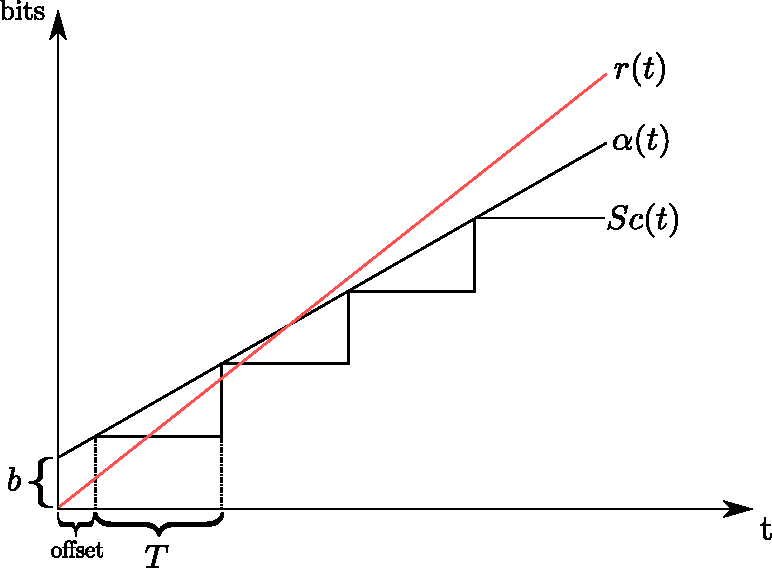
\includegraphics[width = .4\textwidth]{arrivalCurves}
  \caption{$Sc(t)$ is the staircase arrival curve, $\alpha(t)$ is the affine model arrival curve and $r(t)$ is the service curve defined by the capabilities of the CAN Bus.}
  \label{fig:arrivalCurves}
\end{figure}

The affine arrival model in relation to the real unknown arrival function is given by
\begin{flalign}
  R(t) \leq \alpha (t) &= b + \frac{P}{T} t &
\end{flalign}
%
\begin{where}
  \va{\alpha}{is the affine model arrival curve}{}
  \va{b}{is the crossing of the affine curve with the y-axis}{}
\end{where}
%
The relation between both models and the unknown real arrival function is then given by
\begin{flalign}
  R &\leq Sc \leq \alpha &
\end{flalign}

\subsection{Wheel Sensor Data Arrival}
The staircase arrival model for the wheel sensor data is
\begin{flalign}
  Sc_\mathrm{w} (t) &= \left\lceil \frac{t - \cancelto{0}{\mathrm{offset}} \ \ \ }{T_\mathrm{w}} \right\rceil \times P_\mathrm{w}& \\
  Sc_\mathrm{w} (t) &= \left\lceil \frac{t}{0.04} \right\rceil \times 160 \ \ ,&
\end{flalign}
where $P_\mathrm{w} = 20\times 8$ since the packet size is \SI{20}{B}, which means that \SI{160}{b} arrive at each time interval, $T = 0.04$. The time offset is set to zero in order to model for worst case.
%
%\begin{where}
%  \va{Sc_\mathrm{w} (t)}{is the staircase model arrival curve for the wheel sensor data.}{}
%  \va{t}{is the time.}{}
%  \va{\mathrm{offset}}{is the time offset measured from $t = 0$ to first packet arrival.}{}
%  \va{T_\mathrm{w}}{is the period time for packet arrivals from the wheel sensors.}{}
%  \va{P_\mathrm{w}}{is the packet size containing the wheel sensor data.}{}
%\end{where}
%
%
The affine arrival model for the wheel sensor data is
\begin{flalign}
  \alpha_\mathrm{w} (t) &= b + \frac{P_\mathrm{w}}{T_\mathrm{w}} t & \\
  \alpha_\mathrm{w} (t) &= 160 + \frac{160}{0.04} t  = 160 + 6.4 t \ \ ,&
\end{flalign}
where $b = P_\mathrm{w} = 160$ since the time offset is set to zero to model worst case.
%
%\begin{where}
%  \va{\alpha_\mathrm{w} (t)}{is the affine model arrival curve for the wheel sensor data}{}
%  \va{b}{is the crossing of the affine curve with the y-axis}{}
%\end{where}
%
%

\subsection{Electronic Speed Control (ESC) Data Arrival}
The staircase arrival model for the wheel sensor data is
\begin{flalign}
  Sc_\mathrm{ESC} (t) &= \left\lceil \frac{t - \cancelto{0}{\mathrm{offset}} \ \ \ }{T_\mathrm{ESC}} \right\rceil \times P_\mathrm{ESC}& \\
  Sc_\mathrm{ESC} (t) &= \left\lceil \frac{t}{0.4} \right\rceil \times 64 \ \ ,&
\end{flalign}
where $P_\mathrm{ESC} = 8\times 8$ since the packet size is \SI{8}{B}, which means that \SI{64}{b} arrive at each time interval, $T = 0.4$. The time offset is again set to zero in order to model for worst case.
%
%\begin{where}
%  \va{Sc_\mathrm{w} (t)}{is the staircase model arrival curve for the wheel sensor data.}{}
%  \va{t}{is the time.}{}
%  \va{\mathrm{offset}}{is the time offset measured from $t = 0$ to first packet arrival.}{}
%  \va{T_\mathrm{w}}{is the period time for packet arrivals from the wheel sensors.}{}
%  \va{P_\mathrm{w}}{is the packet size containing the wheel sensor data.}{}
%\end{where}
%
The affine arrival model for the wheel sensor data is
\begin{flalign}
  \alpha_\mathrm{ESC} (t) &= b + \frac{P_\mathrm{ESC}}{T_\mathrm{ESC}} t & \\
  \alpha_\mathrm{ESC} (t) &= 64 + \frac{64}{0.4} t = 64 + 25.6 t \ \ ,&
\end{flalign}
where $b = P_\mathrm{ESC} = 64$ since the time offset is set to zero to model worst case.

\begin{figure}[H]
	\captionbox
	{
		Arrival curves for the four wheels and service curve for the CAN-bus.
		\label{fig:ArrivalCurvesWheels}
	}
	{
		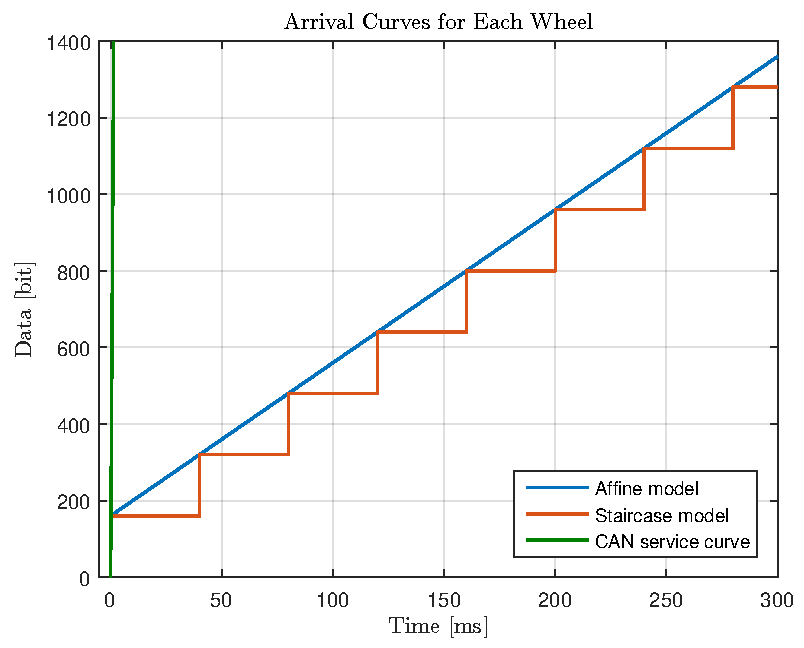
\includegraphics[width=.46\textwidth]{figures/ArrivalCurvesWheels}
	}
	\hspace{5pt}
	\captionbox
	{
		Arrival curves for the ESC and service curve for the CAN-bus.
		\label{fig:ArrivalCurvesESC}
	}
	{
		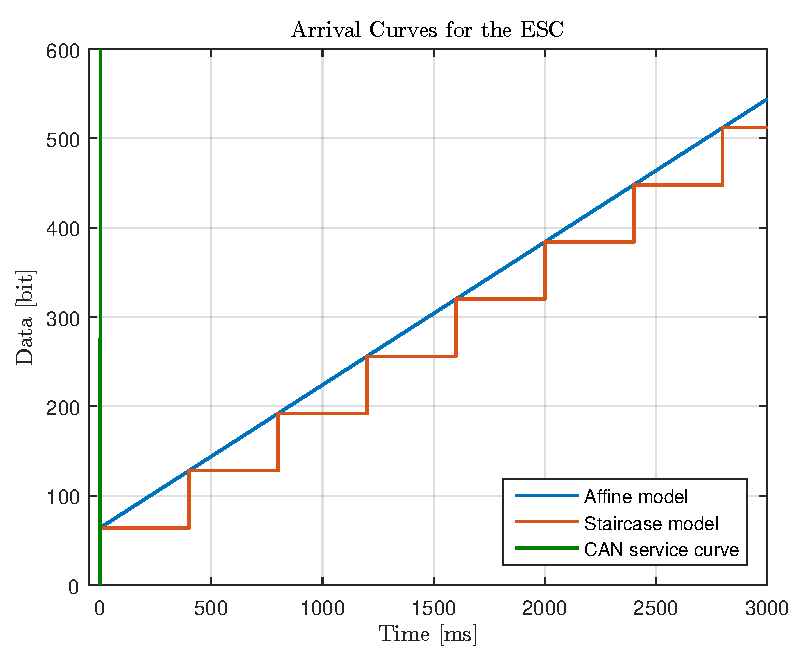
\includegraphics[width=.46\textwidth]{figures/ArrivalCurvesESC}
	}
\end{figure}
\section{Token Filter}

\begin{figure}[H]
	\includegraphics[width = .4\textwidth]{tokenFilter}
	\caption{Token filter}
	\label{fig:tokenFilter}
\end{figure}
%
\begin{figure}[H]
	\captionbox
	{
		Arrival curves for the Multimedia and service curve for the CAN-bus.
		\label{fig:ArrivalCurvesMultimedia}
	}
	{
		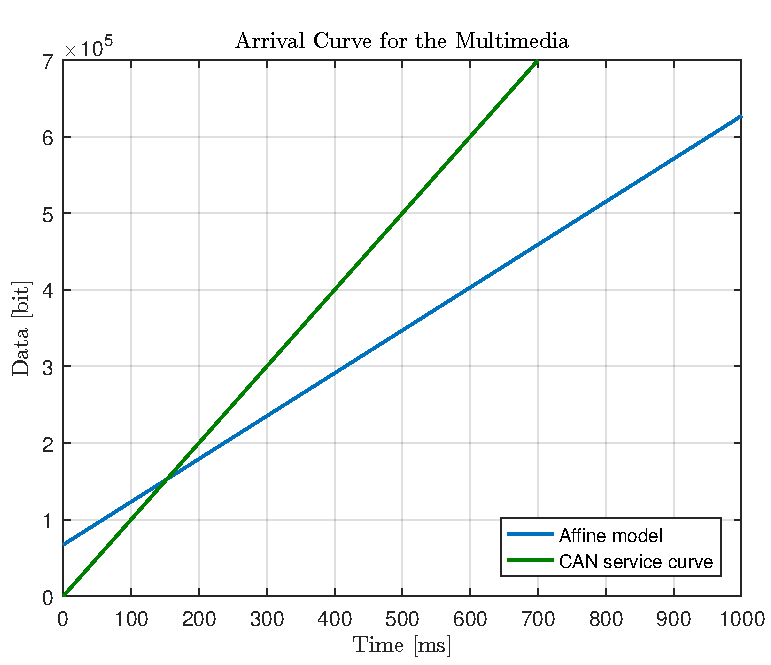
\includegraphics[width=.46\textwidth]{figures/ArrivalCurvesMultimedia}
	}
	\hspace{5pt}
	\captionbox
	{
		Arrival curves for the RC and service curve for the CAN-bus.
		\label{fig:ArrivalCurvesRC}
	}
	{
		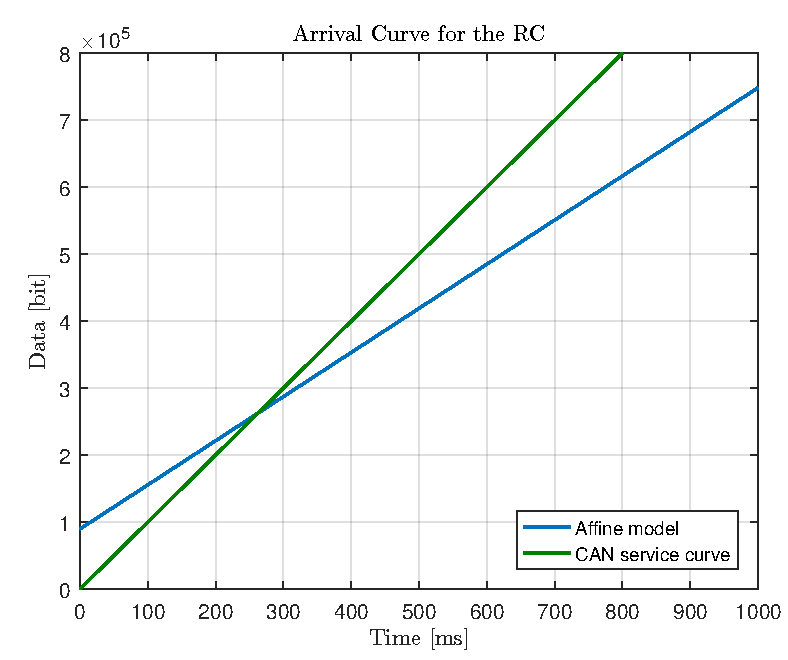
\includegraphics[width=.46\textwidth]{figures/ArrivalCurvesRC}
	}
\end{figure}
%
\subsection{Service Model}
The curve for the service model, $r(t)$, is seen in \autoref{fig:arrivalCurves}. The model is linear and defined by the capabilities of the CAN Bus with a rate of \SI{1}{Mbps}.


\section{Reliability}
The failure rate can be translated to be in fails/year. This is done in \autoref{eq:failrate}.

\begin{flalign}
	\lambda=\frac{1 \mathrm{fails}}{2\cdot10^6\mathrm{h}}\cdot\frac{8760 \mathrm{h}}{1\mathrm{year}}=\frac{1 \mathrm{fails}}{288.3\mathrm{year}}
	\label{eq:failrate}
\end{flalign}

The lifetime of the car can be expressed by its probability density function seen in \autoref{eq:carpdf}.
\begin{flalign}
	f_{\mathrm{car}}(t)=
	\begin{cases}
		\frac{1}{10} & \text{if } t\in[5,15]\\
		0               & \text{otherwise}
	\end{cases}
	\label{eq:carpdf}
\end{flalign}
\subsection{Case 1}
For the first case, the reliability, cumulative and probability functions for the lifetime of the network can be found. The first one obtained is the reliability function and it is found by multiplying the individual reliabilities for the two switches as they are connected in series, see \autoref{fig:case1}, and they have independent probabilities of failing. 
\begin{figure}[H]
	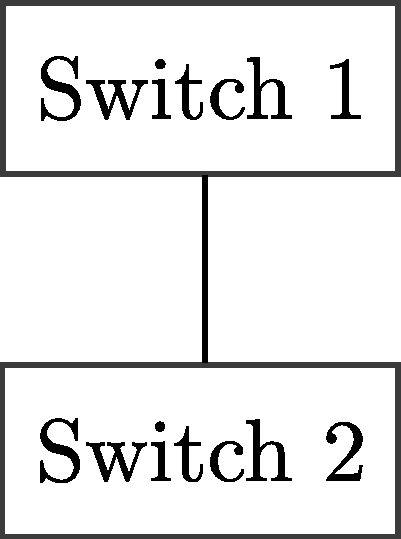
\includegraphics[width = .2\textwidth]{case1}
	\caption{Switch diagram for case 1}
	\label{fig:case1}
\end{figure}

\begin{flalign}
	R_{\mathrm{n}}(t)&=R_1(t)R_2(t)=e^{-\lambda t}e^{-\lambda t}=e^{-2\lambda  t}\label{eq:reliabilitycase1} \\
	F_{\mathrm{n}}(t)&=1-R_{\mathrm{n}}(t)=1-e^{-2\lambda t} \label{eq:cumulativecase1}  \\
	f_{\mathrm{n}}(t)&={F^{\prime}}_{\mathrm{n}}=-2 \lambda e^{{-2\lambda t}} \label{eq:probabilitycase1}  
\end{flalign}

To find the probability of the network failing before the rest of the car does, a double integration is performed from 5 to 15 for and from 0 to $t_{\mathrm{c}}$, where $t_{\mathrm{c}}$ is the time in which the car fails. \autoref{eq:integralcase1} shows the performed computation.


\begin{flalign}
	P(t_\mathrm{n}-t_\mathrm{c})&=\int_{5}^{15}\left[\int_{0}^{t_{\mathrm{c}}}f_{\mathrm{n}}(t)f_{\mathrm{c}}(t)dt_{\mathrm{n}}\right]dt_{\mathrm{c}}\label{eq:integralcase1}
\end{flalign}

The result of this integral gave a probability of 0.0668 of the network failing before the rest of the car.
\subsection{Case 2 a}
In case 2 a, one of the switches is duplicated as seen in \autoref{fig:case2a}. Even though the method is the same, the reliability, cumulative and probability functions change as now there is one more switch in the network. 
\begin{figure}[H]
	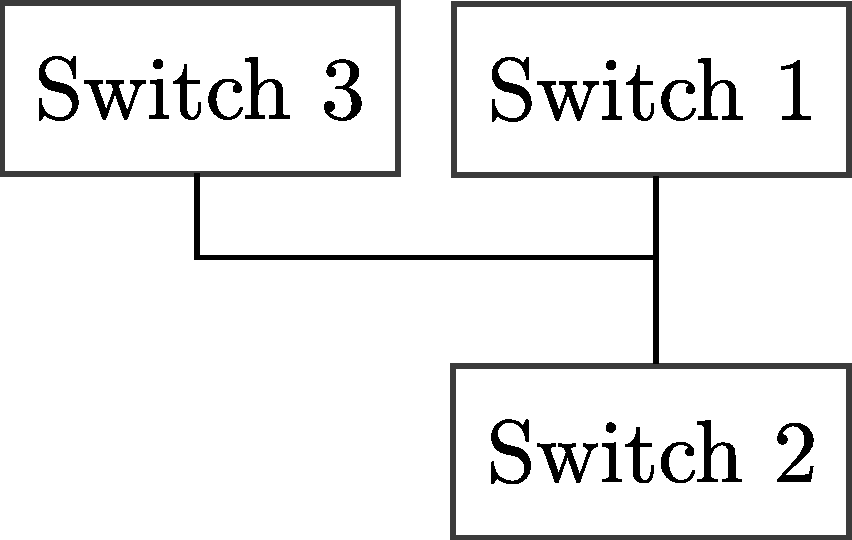
\includegraphics[width = .4\textwidth]{case2a}
	\caption{Switch diagram for case 2 a}
	\label{fig:case2a}
\end{figure}
\begin{flalign}
	R_{\mathrm{n}}(t)&=R_2(R_1(t)+R_3(t)-R_1(t)R_3(t))=e^{-\lambda t}\left(2e^{-\lambda t}-e^{-2\lambda  t}\right)= 2e^{-2\lambda  t} - e^{-3 \lambda t} \label{eq:reliabilitycase2a} \\
	F_{\mathrm{n}}(t)&=1-R_{\mathrm{n}}(t)= 1-2e^{-2\lambda  t} + e^{-3 \lambda t}\label{eq:cumulativecase2a}  \\
	f_{\mathrm{n}}(t)&={F^{\prime}}_{\mathrm{n}}=4 \lambda e^{{-2\lambda t}} -3 \lambda e^{{-3\lambda t}}  \label{eq:probabilitycase2a}  
\end{flalign}

The integral is done in the same way as seen in \autoref{eq:integralcase1} but in this case the expression for $f_{\mathrm{n}}$ is different. The result obtained is 0.00346.

\subsection{Case 2 b}
In the last case, both switches are duplicated. The structure is shown in \autoref{fig:case2b}. Again, the reliability, cumulative and probability functions change and they need to be re-calculated taking into account the new combination of series and parallel connection. This is shown in \autoref{eq:reliabilitycase2b} and \ref{eq:cumulativecase2b} and \ref{eq:probabilitycase2b}.
\begin{figure}[H]
	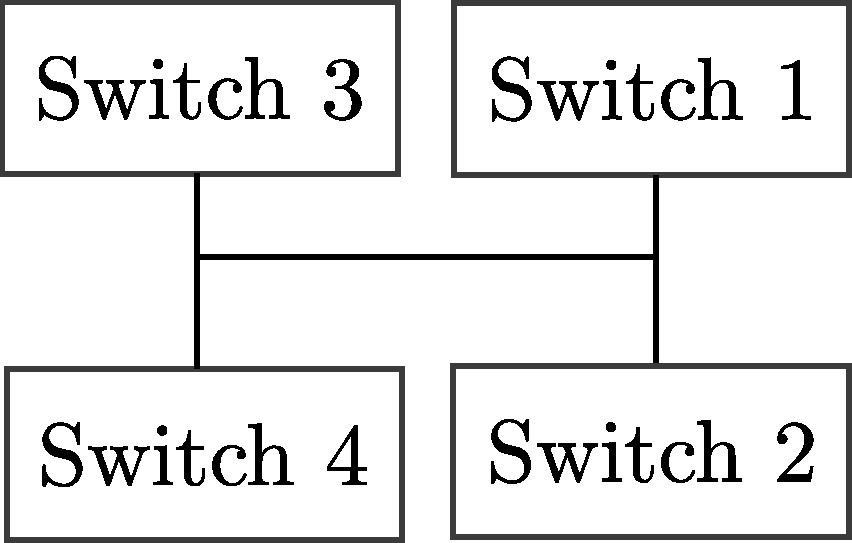
\includegraphics[width = .4\textwidth]{case2b}
	\caption{Switch diagram for case 2 b}
	\label{fig:case2b}
\end{figure}
\begin{flalign}
	R_{\mathrm{n}}(t)&=(R_1(t)+R_3(t)-R_1(t)R_2(t))(R_2(t)+R_4(t)-R_2(t)R_4(t))=\label{eq:reliabilitycase2b} \\
			&\left(2e^{-\lambda t}-e^{-2\lambda  t}\right)\left(2e^{-\lambda t}-e^{-2\lambda  t}\right)=\left(4e^{-2\lambda t}-4e^{-3\lambda t}+e^{-4\lambda t}\right)\nonumber\\
	F_{\mathrm{n}}(t)&=1-R_{\mathrm{n}}(t)=1-e^{-2\lambda t} \label{eq:cumulativecase2b}  \\
	f_{\mathrm{n}}(t)&={F^{\prime}}_{\mathrm{n}}=-2 \lambda e^{{-2\lambda t}} \label{eq:probabilitycase2b}  
\end{flalign}

The new probability density function is used to find the probability of the network failing before the car does in the same way as with the previous two cases. See \autoref{eq:integralcase1}. The result obtained for this case is 0.0025. 

It can be seen that the failure probability is reduces the more redundant components are present in the network.


%
\begin{figure}[H]
  \captionbox
  {
    Arrival curves for the four wheels and service curve for the CAN-bus.
    \label{fig:ArrivalCurvesWheels}
  }
  {
    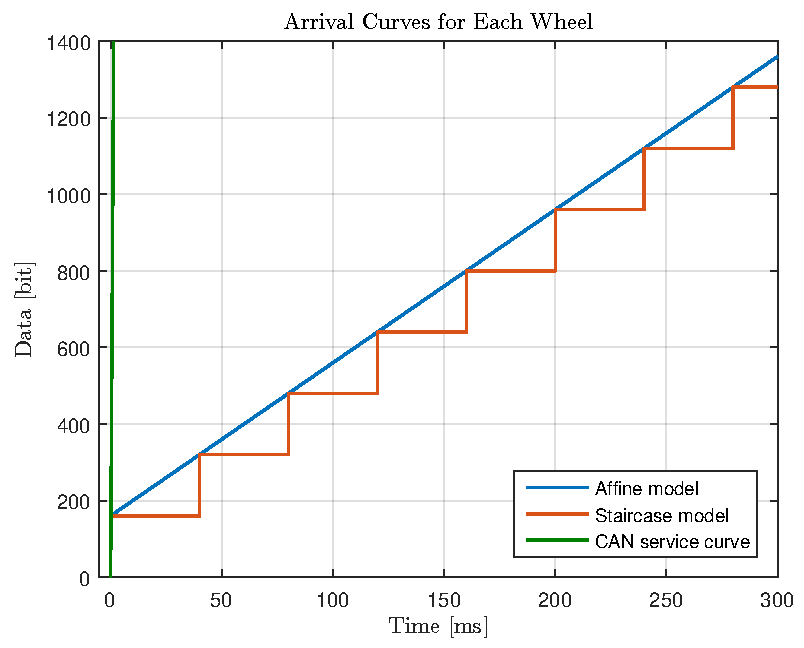
\includegraphics[width=.46\textwidth]{figures/ArrivalCurvesWheels}
  }
  \hspace{5pt}
  \captionbox
  {
    Arrival curves for the ESC and service curve for the CAN-bus.
    \label{fig:ArrivalCurvesESC}
  }
  {
    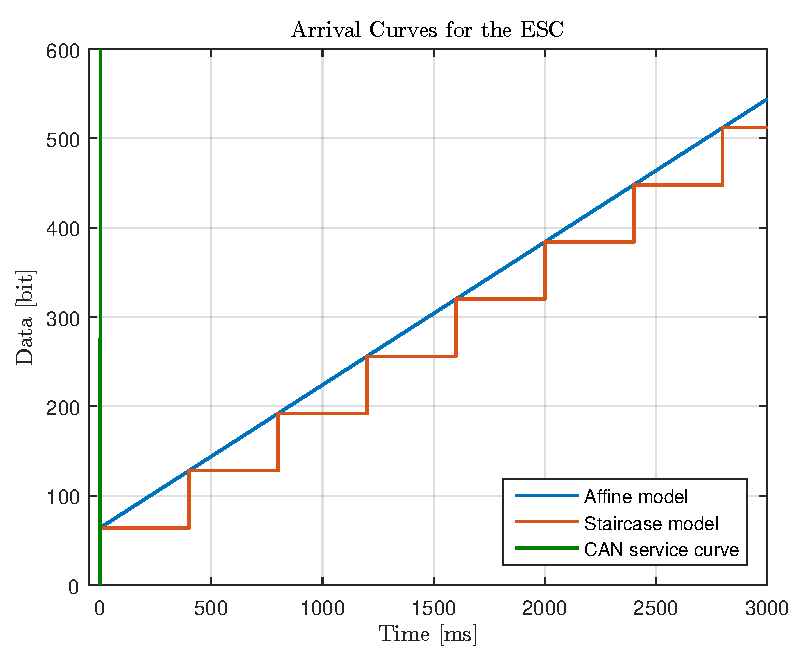
\includegraphics[width=.46\textwidth]{figures/ArrivalCurvesESC}
  }
\end{figure}
%
%
\begin{figure}[H]
  \captionbox
  {
    Arrival curves for the Multimedia and service curve for the CAN-bus.
    \label{fig:ArrivalCurvesMultimedia}
  }
  {
    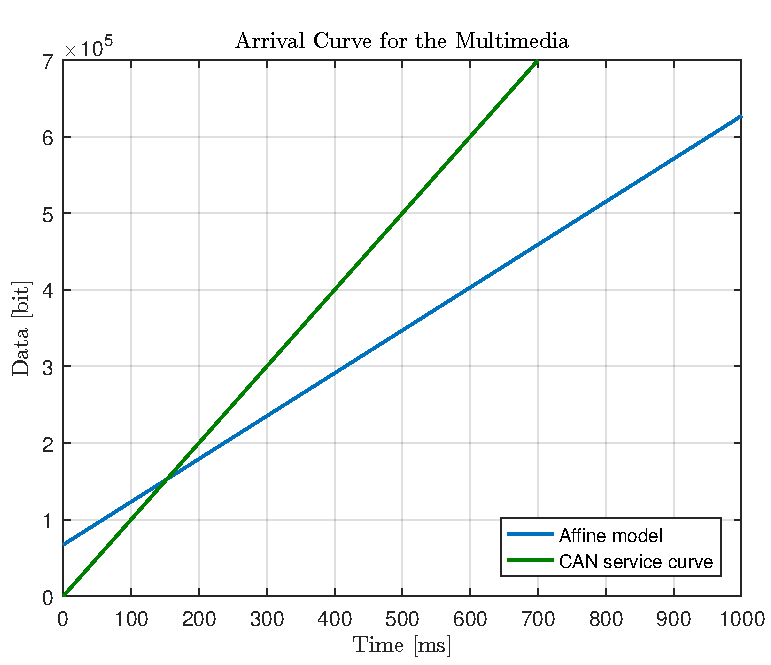
\includegraphics[width=.46\textwidth]{figures/ArrivalCurvesMultimedia}
  }
  \hspace{5pt}
  \captionbox
  {
    Arrival curves for the RC and service curve for the CAN-bus.
    \label{fig:ArrivalCurvesRC}
  }
  {
    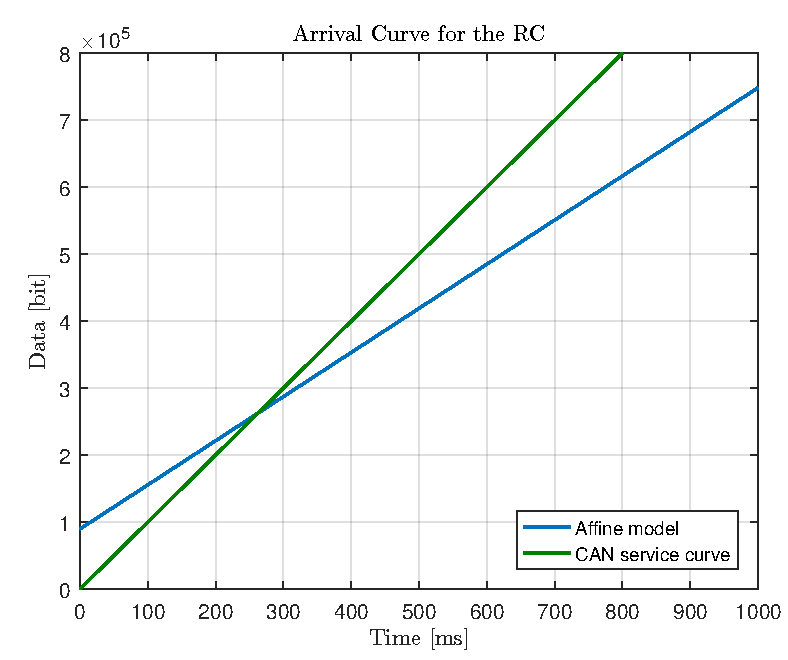
\includegraphics[width=.46\textwidth]{figures/ArrivalCurvesRC}
  }
\end{figure}
%


\printbibliography
%\listoffixmes
\end{document}